\documentclass{homework}
\usepackage{setspace}
\usepackage{enumitem}

\author{Shu Wan, ASUID 1226038322}
\class{CSE 691: Topics in Reinforcement Learning}
\date{\today}
\title{Homework Assignment 1}
%\address{Bayt El-Hikmah}

\graphicspath{{./media/}}

\setlength{\parskip}{1em}

\begin{document} \maketitle

\question Computational Exercise - Traveling Salesman Problem

Consider a modified version of the four-city traveling salesman problem of Example
1.2.3, where there is a fifth city E. The intercity travel costs are shown in
Fig. \ref{fig:1}, which also gives the solutions to parts (a), (b), and (c).

\begin{figure}[h]
    \centering
    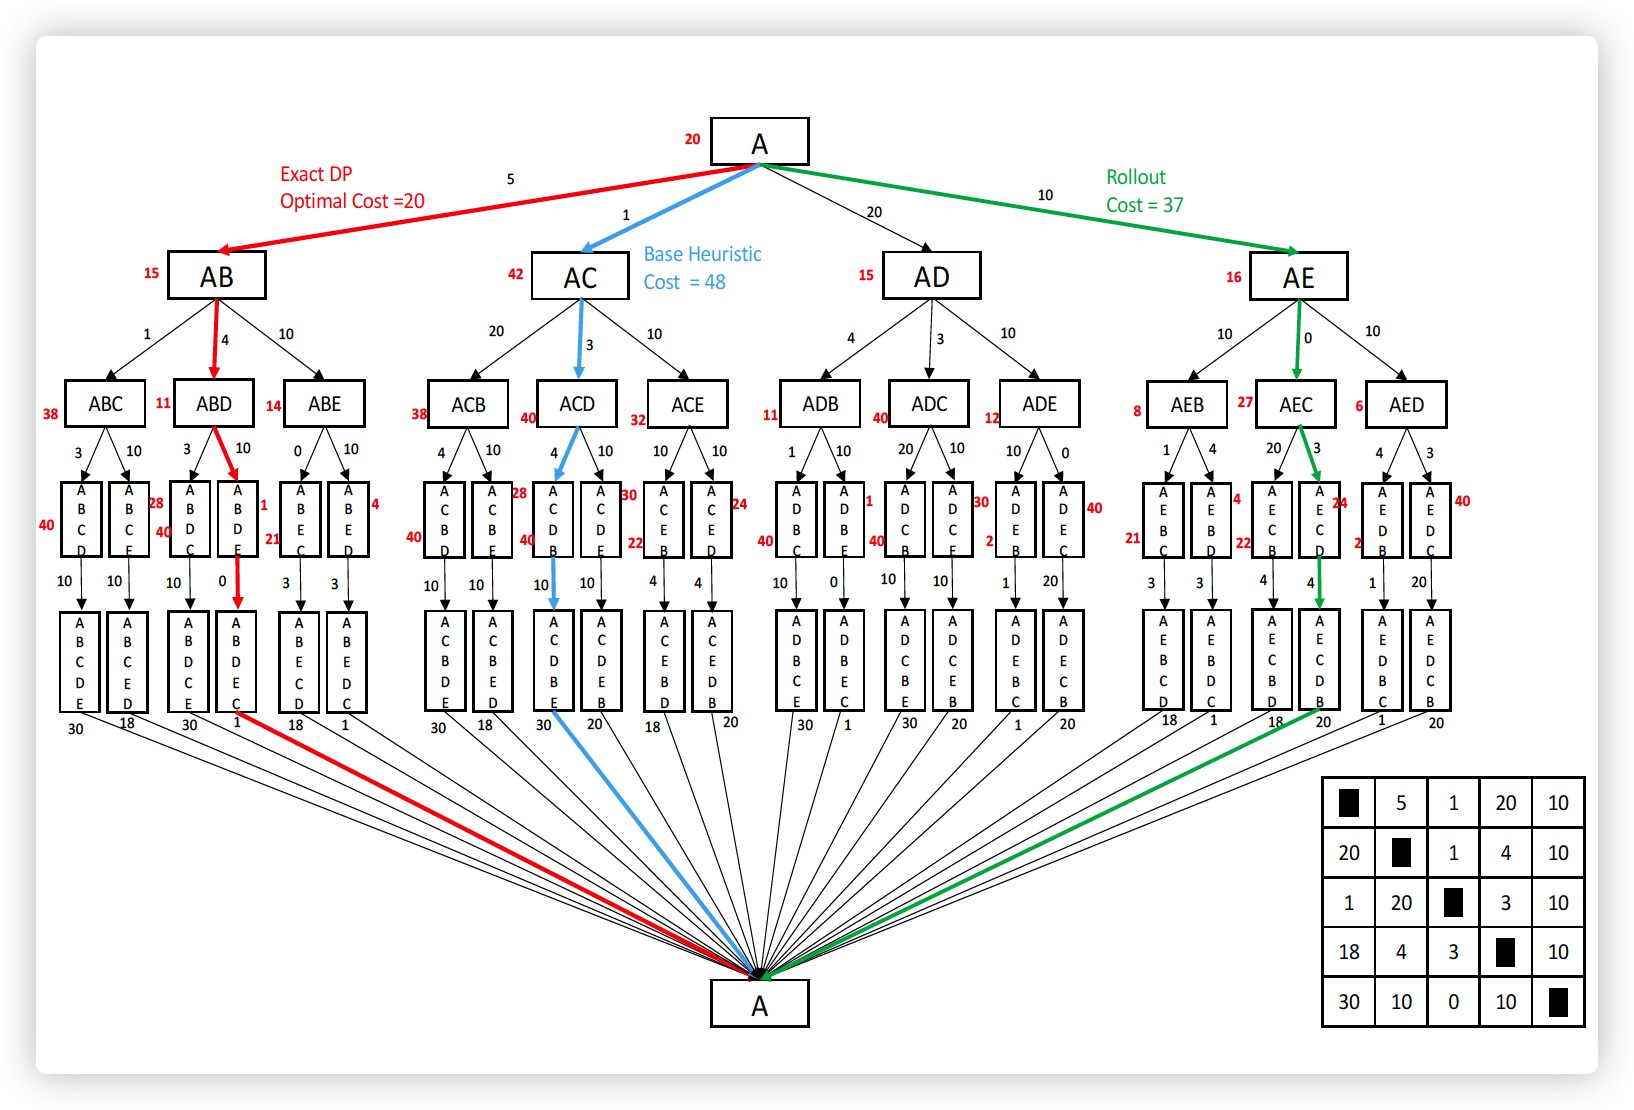
\includegraphics[width=\linewidth]{media/tsp.jpg}
    \caption{Solution of parts (a), (b), and (c) of Exercise 1 A 5-city traveling salesman problem illustration of rollout with the nearest neighbor base heuristic.}
    \label{fig:1}
\end{figure}

\begin{enumerate}[label=(\alph*)]
\setlength{\itemsep}{3pt}
    \item Use exact DP with starting city A to verify that the optimal tour is ABDECA
with cost 20.
\item Verify that the nearest neighbor heuristic starting with city A generates
the tour ACDBEA with cost 48.
\item Apply rollout with one-step lookahead minimization, using as base heuristic
the nearest neighbor heuristic. Show that it generates the tour AECDBA
with cost 37.

\item Apply rollout with two-step lookahead minimization, using as base heuristic
the nearest neighbor heuristic. This rollout algorithm operates as follows.
For $k = 1, 2, 3$, it starts with a $k$-city partial tour, it generates every possible
two-city addition to this tour, uses the nearest neighbor heuristic to
complete the tour, and selects as next city to add to the $k$-city partial tour
the city that corresponds to the best tour thus obtained (only one city is
added to the current tour at each step of the algorithm, not two). Show
that this algorithm generates the optimal tour.

\item Estimate roughly the complexity of the computations in parts (a), (b), (c), and (d), assuming a generic $N$-city traveling salesman problem. 
\end{enumerate}

\newpage

\section*{Solution}

(a) 

\textbf{Illustration of the algorithm}

We follow the Exact DP strategy described in Eq (1.4, 1.5) to find the optimal tour path.

Starting from the terminal node (A), the shortest path is highlighted in red with cost 1. There are 6 optimal paths for state 5 sub-problem (Fig \ref{fig:tsp1-1}).
\begin{figure}[ht]
    \centering
    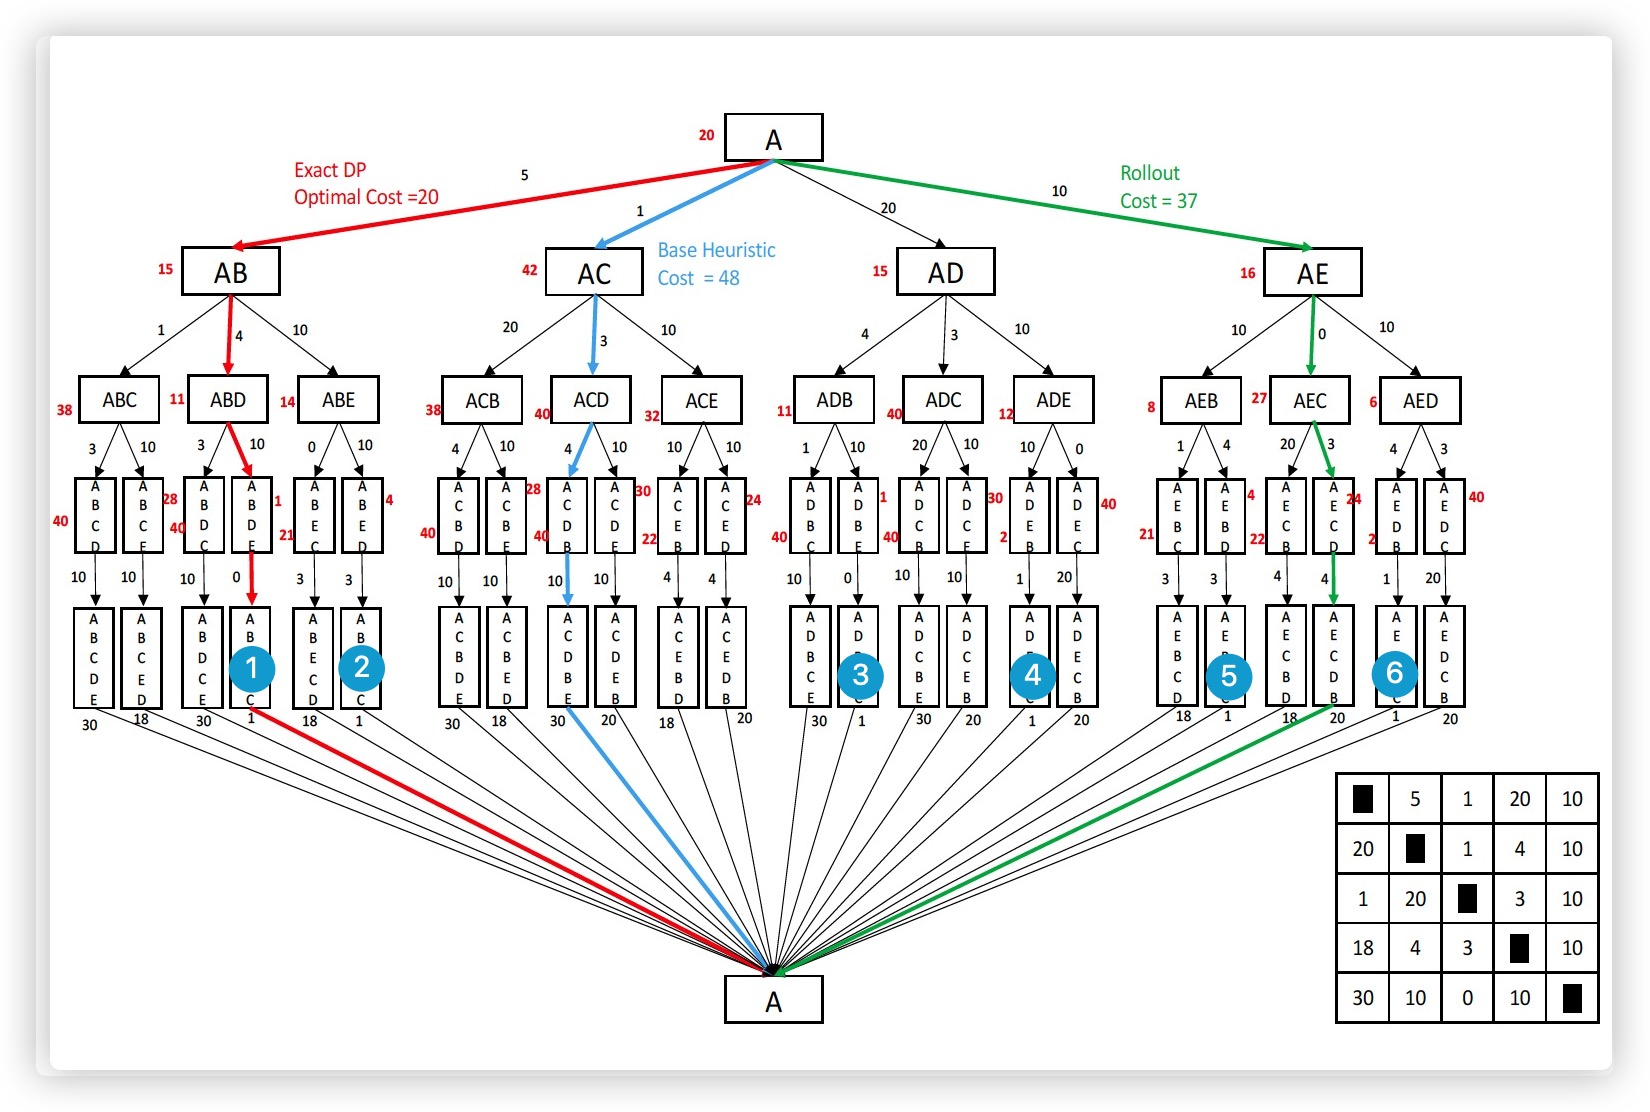
\includegraphics[width=0.6\linewidth]{media/tsp1-1.jpg}
    \caption{State 5 subproblem}
    \label{fig:tsp1-1}
\end{figure}

For state 4 sub-problem, there are two optimal paths with cost 1 (Fig \ref{fig:tsp1-2}).

\begin{figure}[ht]
    \centering
    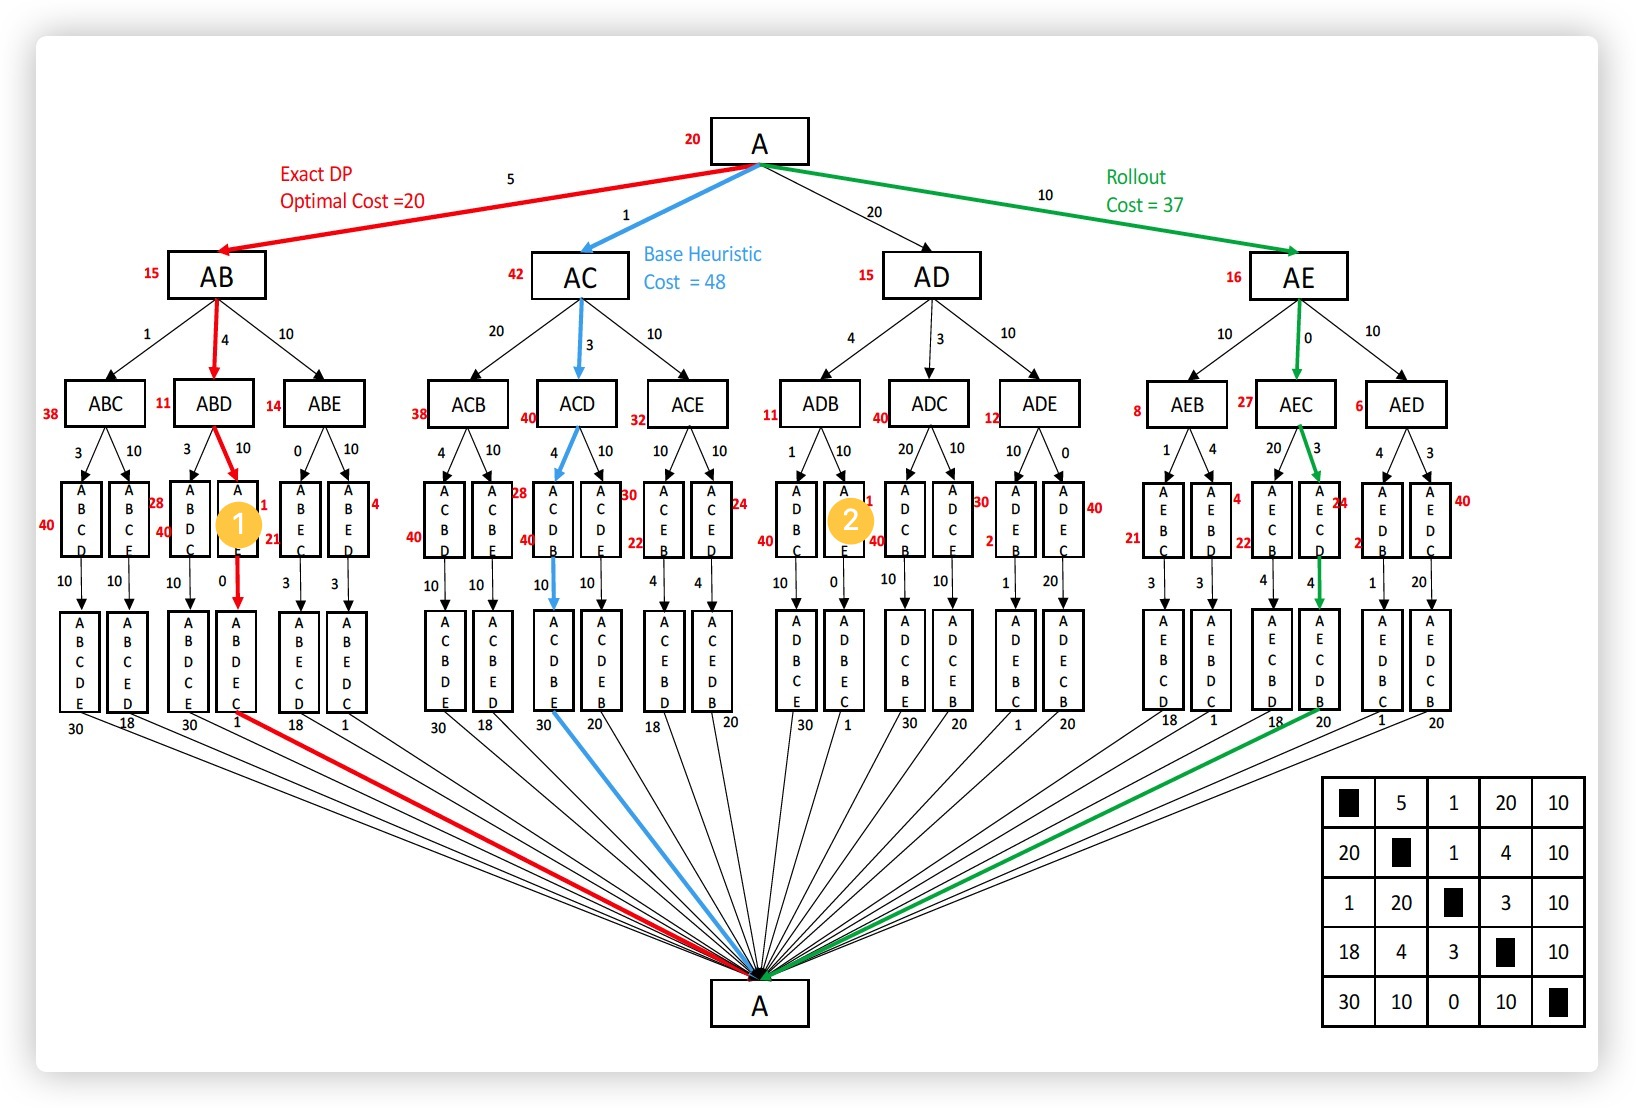
\includegraphics[width=0.6\linewidth]{media/tsp1-2.jpg}
    \caption{State 4 subproblem}
    \label{fig:tsp1-2}
\end{figure}

For state 3 sub-problem, there is one optimal path with cost 8 (Fig \ref{fig:tsp1-3}).

\begin{figure}[ht]
    \centering
    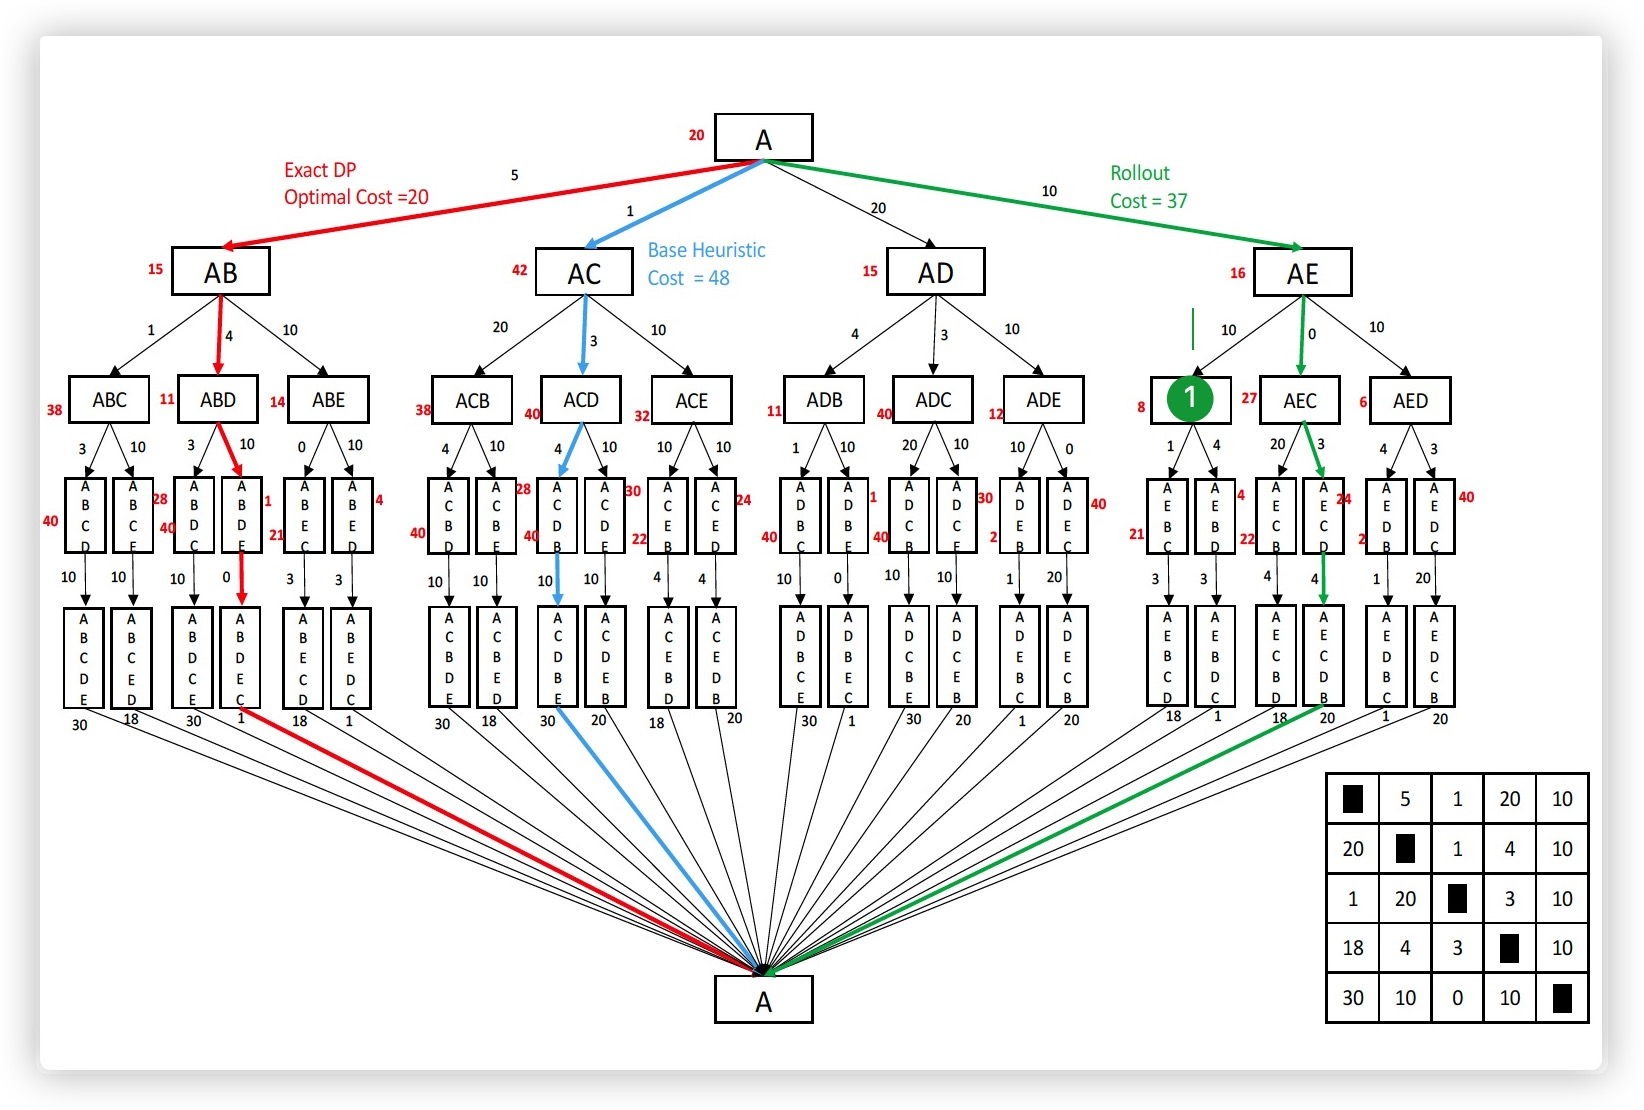
\includegraphics[width=0.6\linewidth]{media/tsp1-3.jpg}
    \caption{State 3 subproblem}
    \label{fig:tsp1-3}
\end{figure}

For state 2 sub-problem, there are two optimal paths with cost 15 (Fig \ref{fig:tsp1-4}).
\begin{figure}[ht]
    \centering
    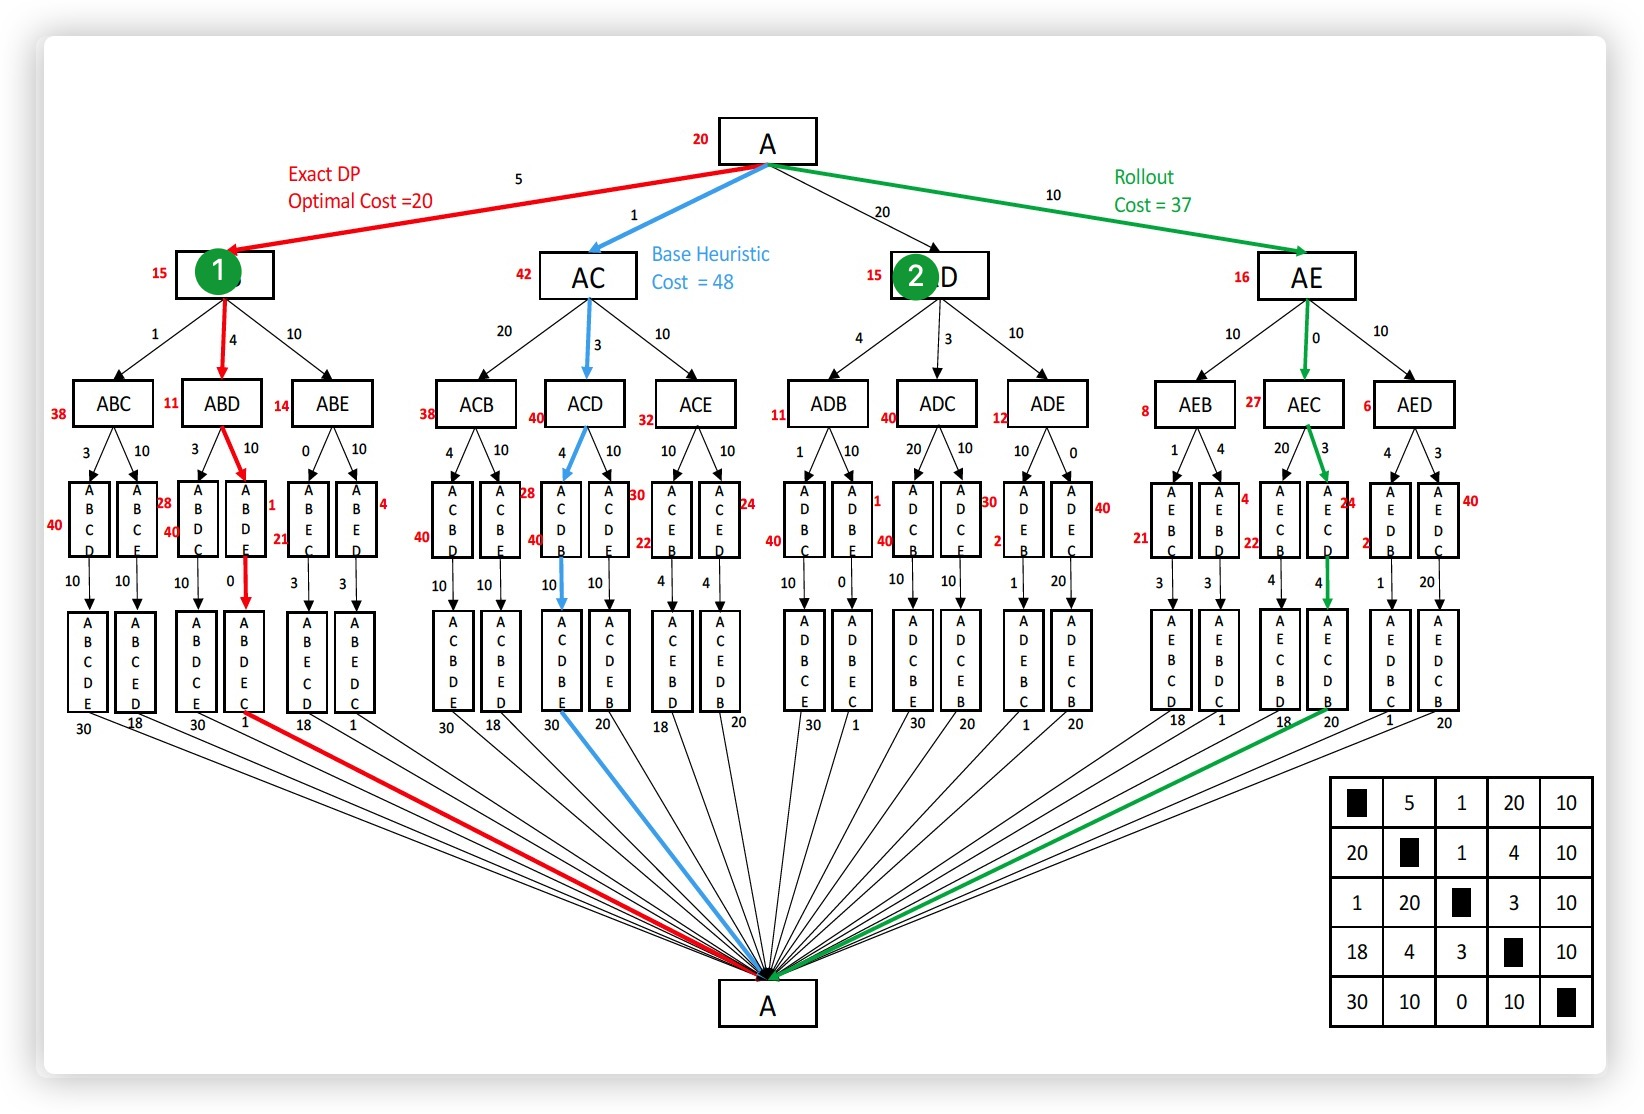
\includegraphics[width=0.6\linewidth]{media/tsp1-4.jpg}
    \caption{State 2 subproblem}
    \label{fig:tsp1-4}
\end{figure}

For the state 0 sub-problem, the optimal path is the one colored in red with the cost of 20. Then the algorithm travels forward to construct the optimal action sequence: ABDECA.

(b)

\textbf{Illustration of the algorithm}

In nearest neighbor heuristic, the algorithm chooses the sub-optimal control sequence by minimizing the next transition cost (greedy). At city A, the nearest neighbor is C with cost 1. At states AC, the closest city is D with cost 3. At state ACD, city B is the next step with the lowest cost 4. For the next step, E is the only option, and finally travels back to city A with cost 30.
In this case, the sub-optimal control sequence is A - C - D - B - E - A. Each control achieves minimal cost in each step. The path highlight in blue in Fig \ref{fig:1}. The total cost is 1 + 3 + 4 + 10 + 30 = 48.

(c)

\textbf{Illustration of the algorithm}

\begin{enumerate}
    \item The first step is determined by comparing all subsequent tail costs using base policy illustrated in part (b). There are four stage 1 states, AB, AC, AD, AE. For each state, the sub-optimal routes using base policy are ABCDEA with cost 49, ACDBEA with cost 48, ADCEBA with cost 63, and AECDBA with cost 37. 
AE is chosen as the first stage state for its tail sub-optimal tour AECDBA has the minimal cost.
\item  Moving to the next stage, the algorithm compares the tail tour costs for AEB, AEC, and AED. The corresponding tours are AEBCDA with cost 42, AECDBA with cost 37, AEDCBA with cost 63. The algorithm moves to AEC because AECDBA has the lowest cost.
\item At AEC, the algorithm compares nearest neighbor heuristic tours of two states AECB and AECD. The algorithm moves to D for its least cost (AECBDA with cost 42 and AECDBA with cost 37).
\item For the last step, only one option is left and the final tour path is AECDBA with cost 37.
\end{enumerate}
 

(d)

\textbf{Illustration of the algorithm}

\begin{enumerate}
    \item \textbf{k = 1}
    
    Starting with all possible three-city partial tours (12 in total). Complete the tour using base heuristics and pick the partial tour with minimal cost.
    \begin{enumerate}
        \item ABCDEA: 5 + 1 + 3 + 10 + 30 = 49
        \item ABDCEA: 5 + 4 + 3 + 10 + 30 = 52
        \item ABECDA: 5 + 10 + 0 + 3 + 18 = 36
        \item ACBDEA: 1 + 20 + 4 + 10 + 30 = 65
        \item ACDBEA: 1 + 3 + 4 + 10 + 30 = 48
        \item ACEBDA: 1 + 10 + 1 + 4 + 18 = 34
        \item ADBCEA: 20 + 4 + 1 + 1 + 30 = 56
        \item ADCEBA: 20 + 3 + 10 + 10 + 20 = 63
        \item ADECBA: 20 + 10 + 0 + 20 + 20 = 70
        \item AEBCDA: 10 + 10 + 1 + 3 + 18 = 42
        \item AECDBA: 10 + 0 + 3 + 4 + 20 = 37
        \item AEDCBA: 10 + 10 + 3 + 20 + 20 = 63
    \end{enumerate}
    ABECDA has the lowest cost; Move to B
    \item \textbf{k = 2}
    
    All possible partial tours are: ABCD, ABCE, ABDC, ABDE, ABEC, ABED, with the following complete tour costs
    \begin{enumerate}
        \item ABCDEA: 5 + 1 + 3 + 10 + 30 = 49
        \item ABCEDA: 5 + 1 + 10 + 1 + 18 = 35
        \item ABDCEA: 5 + 4 + 3 + 10 + 30 = 52
        \item ABDECA: 5 + 4 + 10 + 0 + 1 = 20
        \item ABECDA: 5 + 10 + 0 + 3 + 18 = 36
        \item ABEDCA: 5 + 10 + 10 + 3 + 1 = 29
    \end{enumerate}
    ABDECA has the lowest cost; Move to D
    \item \textbf{k = 3}
    
    All possible partial tours are: ABDCE, ABDEC with corresponding complete tours ABDCEA and ABDECA. Given previous computation, ABDECA has the least cost.
    The final tour is ABDECA.
\end{enumerate}

The final tour is the same as the exact DP solution. Therefore, two-step minimization generates the optimal routes.

(e)

\textbf{Answer}
For simplicity, we only consider the worst case here, i.e. each city is connected with other cities and costs along all paths are well defined.

\begin{enumerate}
    \item \textbf{Exact DP}
    The total possible routes for a fully connected N-city problem are $$(N-1)+(N-1)(N-2)+\dots+(N-1)(N-2) \dots 2+(N-1)(N-2) \dots 2\cdot 1$$.
    This number is $O(N!)$ in Big-O notation.

    \item \textbf{Nearest neighbor heuristic}

    At stage k, the nearest neighbor heuristic pick the best action among $k-1$ options. Therefore. the total possible comparisons are
     $$(N-1)+(N-2)+\dots+2+1$$
    This number is $O(N^2)$.

    \item \textbf{$k$-step lookahead}
    At each stage $k$, for $k < N -k$, the algorithm runs neighbor heuristic $N-k$ times. The total computation is 
    $$(N-1)*((N-2)+\dots+1) + (N-2)*((N-3)+\dots+1) + \dots + (N-k)*((N-k-1)+\dots+1)$$,
    which equivalent to $O(N^4)$ in big-oh notation.
\end{enumerate}


% citations
% \bibliographystyle{plain}
% \bibliography{citations}

\end{document}